\documentclass[12pt, a4paper]{article}
\usepackage[margin = 1in, top=1.3in]{geometry}
\usepackage[english]{babel}
\usepackage[utf8]{inputenc}
\usepackage{fancyhdr}
\usepackage[fleqn]{amsmath}
\usepackage{mathtools}
\usepackage{tabto}
\usepackage{bm}
\usepackage{graphicx}
\graphicspath{{./images/}}
\usepackage[font=small,labelfont=bf]{caption}
 
\pagestyle{fancy}
\fancyhf{}
\rhead{\small{Shaan Ul Haque(180070053)\\ Samarth Singh (180050090) \\ Niraj Mahajan (180050069)}}
\lhead{CS-663 Assignment-1 : Question 3}
\rfoot{Page 3.\thepage}
 
\begin{document}
\vspace*{-22pt}
\section*{Question 3}
\subsection*{Part A (8 points)}
\quad After performing histogram equalization, the resultant histogram follows the pdf of a Uniform Distribution. After equalizationof the histograms $h_1$ and $h_2$, let the transformed histograms be $q_1$ and $q_2$ in the regions [0,a] and [a,1] respectively. \\ \\
\null\quad Using mass conservation, the transformed histograms can be obtained as:
\begin{align*}
q_1(I) =&\; \frac{\alpha}{a} &\quad; \;\; I \; \epsilon \; [0,a] \tag{1}\\
q_2(I) =&\; \frac{1-\alpha}{1-a} &\quad; \;\; I \; \epsilon \; [a,1] \tag{2}\\
where \; \alpha = \int_0^ah(I).dI
\end{align*}
For these transformed histograms, the mean intensity is given by:
\begin{align*}
Mean\;Intensity =&\; \int_0^aIq_1(I).dI + \int_a^1Iq_2(I).dI \\
\text{Substituting Equations (1), (2)} \\
Mean\;Intensity =&\; \frac{\alpha}{a}\int_0^aIdI + \frac{1-\alpha}{1-a}\int_a^1IdI \\
=&\; \frac{\alpha}{a}\left(\frac{I^2}{2}\right)\bigg|_0^a + \frac{1-\alpha}{1-a}\left(\frac{I^2}{2}\right)\bigg|_a^1 \\
=&\; \frac{\alpha}{a}\left(\frac{a^2}{2}\right) + \frac{1-\alpha}{1-a}\left(\frac{1-a^2}{2}\right) \\
=&\; \frac{\alpha.a}{2} + \frac{(1-\alpha)(1+a)}{2} \\
\Aboxed{Mean\;Intensity =&\; \frac{1 - \alpha + a}{2}} \tag{3}\\
\end{align*}

\subsection*{Part B (2 points)}
\quad Now, since the chosen intensity $a$ is  the median intensity, this means that the weight is divided exactly into two equal parts at $a$. But since the weight upto $a$ was $\alpha$, we have $\alpha = \frac{1}{2}$ \\ 
\null\quad Substituting this value of $\alpha$ in Eqn (3), we get: 
\begin{align*}
Mean\;Intensity =&\; \frac{1 - \alpha + a}{2}\\
=&\; \frac{1 - \frac{1}{2} + a}{2}\\
\Aboxed{Mean\;Intensity =&\; \frac{0.5 + a}{2}} \tag{4}\\
\end{align*}

\subsection*{Part C (5 points)}
\quad Consider an image (grayscale for simplicity) which has a lot of pixels concentrated within a certain intensity range. Say an image has a lot of pixels with low intensity values. \\ 
\null\quad Simple Histogram Equalization (performed globally) tries to adjust these intensity values such that the transformed values are drawn from an Uniform Distribution, keeping the total weight constant. If we apply this method in the case mentioned in the earlier paragraph, it will result in an undesirable stretching of the low intensity pixels towards higher intensities. \\
\null\quad On the other hand, when we divide the histogram into two components according to the median intensity, we basically are isolating the low intensity pixels in our image and reducing the dominating effect they have while equalizing the histograms. This preserves the brightness of the orignal image to a greater extent, while ensuring overall image enhancement.

\subsection*{Part D (10 points)}
\quad Below are the results obtained using the two methods discussed, in two scenarios. As we can see, when the image has a lot of pixels with low intensity, the method with two separate histogram equalizations greatly outperforms the simple histogram equalization. \\ \\ 
Please Turn Over for the images \\
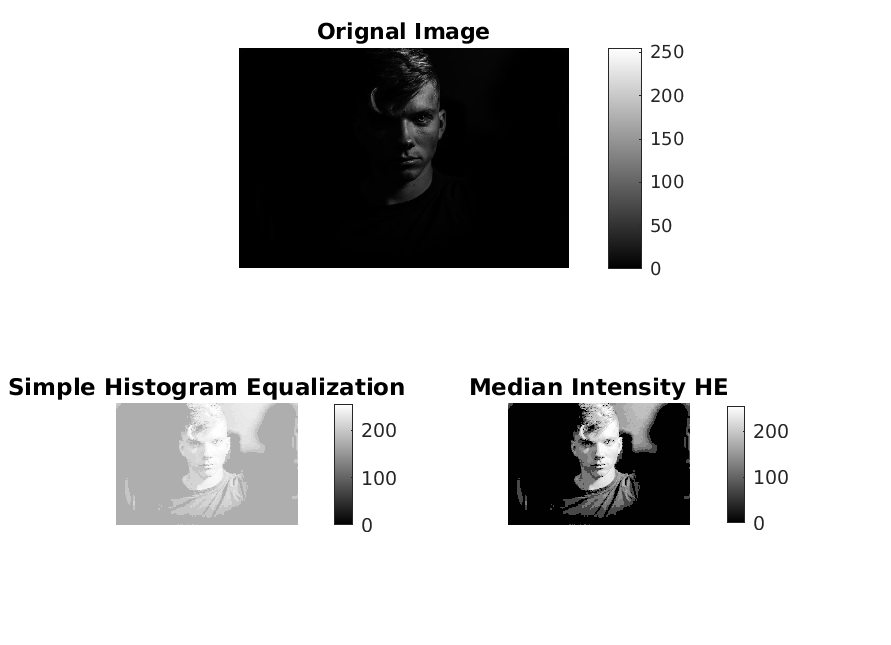
\includegraphics[width=\textwidth]{man.png}
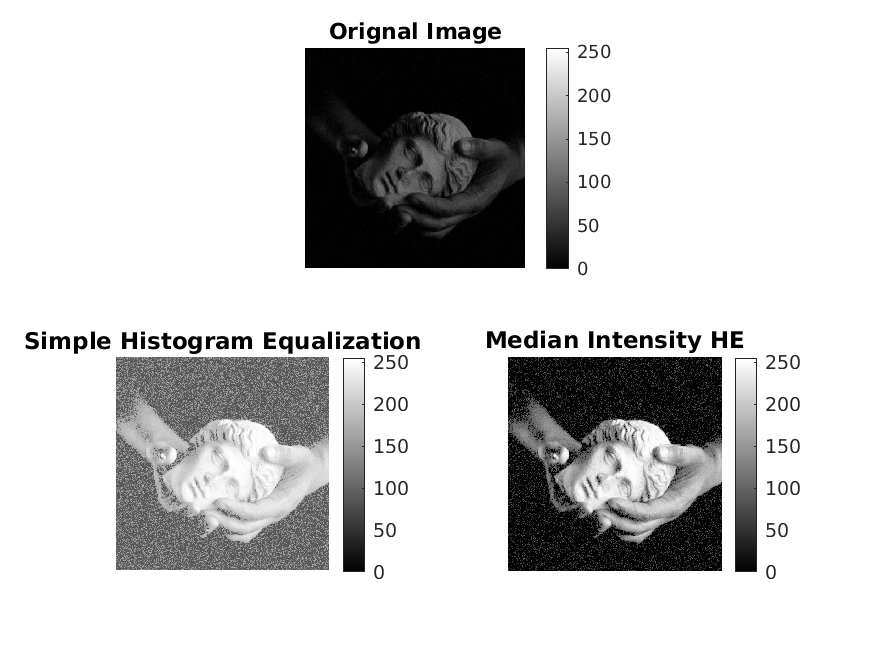
\includegraphics[width=\textwidth]{statue.png}

\subsection*{Part E - Usage of Code}
\begin{itemize}
	\item The main file \textbf{myMainScript.m} simple has function calls to \textbf{myplot.m} for both two test images.
	\item The file \textbf{myplot.m} calls the two different methods to perform histogram equalization from \textbf{histogram\_equalization.m} and \textbf{half\_histogram\_equalization.m} respectively.
\end{itemize}
\end{document}